\documentclass[a4j,twocolumn]{jsarticle}
%\documentclass[a4j,twocolumn,uplatex]{jsarticle}
\usepackage[dvipdfmx]{graphicx}
\usepackage{url}
\usepackage{amsmath}

\setlength{\textheight}{275mm}
\headheight 5mm
\topmargin -30mm
\textwidth 185mm
\oddsidemargin -15mm
\evensidemargin -15mm

%\setlength\intextsep{0pt}
\setlength\textfloatsep{0pt}
\pagestyle{empty}


\begin{document}

\title{粒界構造計算の自動化}
\author{情報科学科 \hspace{5mm} 27014515 \hspace{5mm} 辻脩人}
\date{}
\maketitle

\section{背景}
    西谷研では最安定の粒界エネルギーを第一原理計算で求める研究を行っている.

この研究において,
第一原理計算はVASPという計算ソフトによって自動で行われるが,その前後の作業工程のいくつかが手動で行われている.

手動作業は使い慣れた作業者に取っては,
間違った場合もすぐに気づくことができ,
間違いのケアも迅速に出来るという点では良い.
しかし,初心者が手動の作業を行うと,
途中で何をしているのか分からなくなり,効率が悪くなってしまう

手動による作業の一部を自動で行ったり,
間違いを検出してくれるようなシステムを構築し,
初心者でも簡単に最安定な粒界エネルギーを求められるようにすることが本研究の目的である.

\section{構造最適化の自動化}
構造最適化を行うことで最安定エネルギーを求めるのに必要な最安定構造までの
従来のやり方ではVASPのルーチンを利用して構造最適化を行なっていたが,自動化システム開発にあたりVASPでは時間がかかりすぎるため,原子間ポテンシャルEAMを用いて開発を行った.
数値計算のバイブルNumerical recipeに用意されている標準ルーチンmnbrak\cite{num_recipe}.を利用して,囲い込みを行い,計算点を自動で追加して構造最適化を行なった結果と,手動で構造最適化を行った結果の比較を図\ref{fig:delete_operation}に示した.

近い結果が出ているものの,計算回数を減らせたわけではないので引き続き研究が必要である.

%\section{proposed model}

\section{自動原子削除の実装}

粒界生成において,回転,並びに鏡映操作を行った後の原子配置を図\ref{fig:delete_operation}に示した.
\begin{figure}[htbp]
\begin{center}
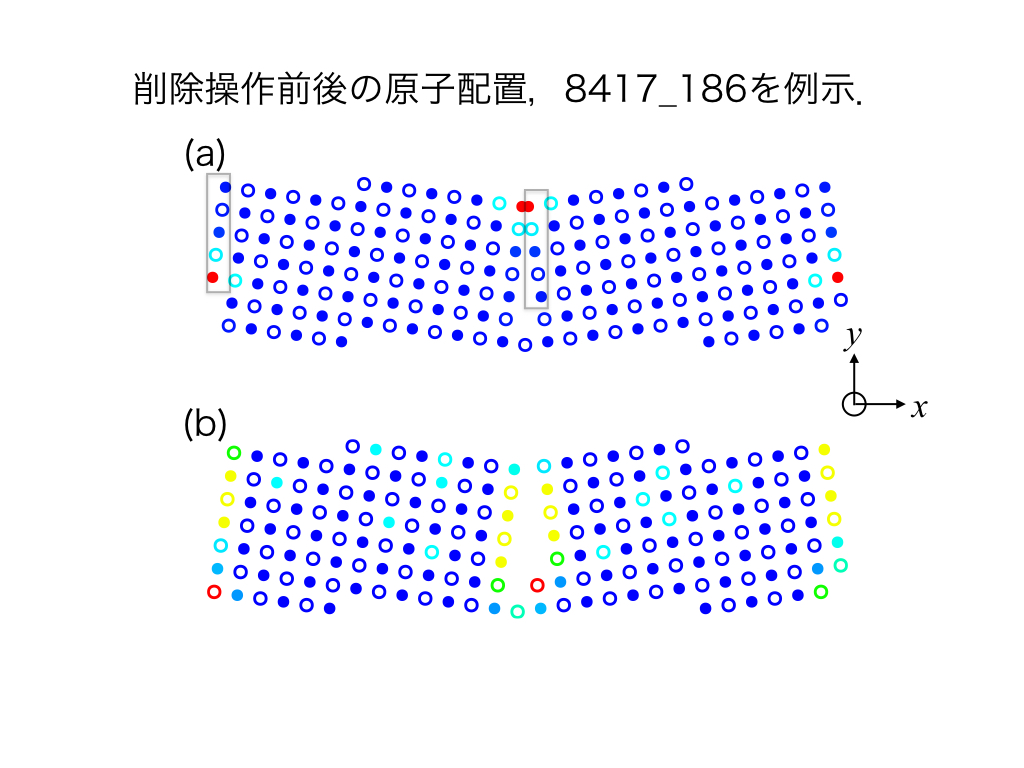
\includegraphics[width=80mm]{auto_delete_002.jpeg}
\caption{削除操作前後の原子配置,8417\_186を例示.}
\label{fig:delete_operation}
\end{center}
\end{figure}

ここでは,8417\_186を例にしている.8417の数字は粒界系全体の構造を表している.それぞれ,x=8,
y=4, z=1およびtan
\(\theta=1/7\)を意味しており,x軸方向に8x2層,y軸方向に4x2層の層を保持している.

削除操作は,この系の端と真ん中あたりにある
粒界近傍において,原子が詰まりすぎているのを解消するために行う操作である.
枠線で囲った領域の原子を削除する.
これまではVestaという表示ソフトを使って,原子サイトナンバーを手動で確認し,
モデル作成司令ファイル(modeler\_8417など)に記述する必要があった.
これを自動化するプログラムを作成した,
初めに作成したEAMのコードを流用したものではうまく原子の選別が出来なかったので,
x座標によって選別を行うように修正し.原子座標の入出力に用いるVASPのPOSCARファイルを直接扱えるクラスを実装した.
これにより削除する原子を細かく設定できるプログラムを開発することが出来たが,削除原子数の指定については断念した.


\section{終わりに}
構造最適化のための囲い込みを自動で行うシステムは,現在行っている手動による指定よりも計算数を劇的に減らすことはできなかった.そこで,粒界近傍の原子削除の自動化を実装した.削除操作は,細かい指定が可能であり,得られたモデルの構造から最適化の最適値を見積もることが期待される.

今後の課題としては
\begin{itemize}
\item 構造最適化ではなく,他の操作を見直すことによるエネルギー計算回数の削減が出来るシステムの開発,
\item 自動原子削除において削除原子数を指定できる機能の追加,
\item 本研究では触れられなかった計算サーバへのファイル転送の自動化
\end{itemize}
が挙げられる.

\vspace{0.5\baselineskip}

{\small\setlength\baselineskip{10pt}	% 参考文献は小さめの文字で行間を詰めてある
\begin{thebibliography}{9}
\bibitem{ReadShockley}W. T. Read Jr., and W. Shockley, "Imperfection in nearly perfect crystals", ed. by W. Shockley, (Wiley, New York, 1952) pp.352--76.
\bibitem{Otsuki} A. Otsuki, J. Materials Science, {\bf 40}(2005), 3219.
\bibitem{TschoppMcdowell} M. A. Tschopp and D. L. Mcdowell, Phil. Mag., {\bf 87}(2007), 3871.
\bibitem{RedBook} 西谷滋人, "固体物理の基礎", (森北, 2006).
\end{thebibliography}
}

\end{document}
